\subsection{変わり目検出の頑健性の定量評価}

課題 7 の変わり目検出については、先の考察で平均 $+k\sigma$ 方式
(方式 (1))・上位 3 ピーク方式(方式 (2))・移動平均基準方式
(方式 (3))の定性的な比較を行い、Detection.mp4 に対しては 3 方式の
検出結果が完全に一致することを述べた。しかしこの一致は「変わり目の
変化量が十分大きい理想的な入力」での結果であり、入力の劣化や
パラメータの変更に対する各方式の挙動の差は定量化されていない。
そこで追加実験(実験ソースは付録の {\tt exp04\_shot\_robustness.py})
として、(1) フレームへのガウスノイズ付加に対する頑健性、
(2) 方式 (1) の係数 $k$ に対する感度、(3) 比較手法としての
グレースケールヒストグラム差分法の追加実装と対比、の 3 点を
定量評価した。対象は Detection.mp4(1920$\times$1080、30 fps、
総フレーム数 322)、正解の変わり目は 3 方式の一致検出と目視確認で
確定したフレーム $\{78, 214, 257\}$ である。実行環境は
macOS(Apple Silicon)、Python 3.13.2、numpy 2.4.4、OpenCV 4.12.0
である。

なお方式 (2) は変わり目の個数を既知とする方式であり、閾値パラメータを
持たず検出数が常に 3 個に固定されるため、閾値方式の頑健性を比較する
本実験の評価対象からは除いた。

\subsubsection{実験条件と評価指標}

ノイズ付加は、グレースケール化後の各フレーム $g_t(x, y)$ に対して
画素ごとに独立なガウスノイズを加え、8 bit の値域に収める操作として
定義した。

\begin{equation}\label{eq:b4-noise}
\tilde{g}_t(x, y) = \mathrm{clip}_{[0, 255]}\bigl(
\mathrm{round}\bigl(g_t(x, y) + n_t(x, y)\bigr)\bigr),
\qquad n_t(x, y) \sim \mathcal{N}(0, \sigma^2)
\end{equation}

ここで $\sigma$ はノイズの標準偏差(画素値スケール)であり、
$\sigma \in \{0, 5, 10, 20, 40\}$ の 5 条件を評価した。乱数は
{\tt np.random.default\_rng(20260702 + $\sigma$)} でシードを固定し、
再現可能とした。変化量系列 $D(t)$ の定義(グレースケール隣接フレーム
差分の絶対値の総和)と検出ロジックは提出プログラムと同一である。

検出結果の評価は、検出フレームと正解フレーム $\{78, 214, 257\}$ を
許容ずれ $\pm 1$ フレームで 1 対 1 に照合(貪欲最近傍)し、
対応の取れた検出を TP、対応のない検出を FP、対応のない正解を FN と
して次式で行った。

\begin{equation}\label{eq:b4-pr}
\mathrm{precision} = \frac{TP}{TP + FP}, \qquad
\mathrm{recall} = \frac{TP}{TP + FN}
\end{equation}

\begin{equation}\label{eq:b4-f1}
F_1 = \frac{2 \cdot \mathrm{precision} \cdot \mathrm{recall}}
{\mathrm{precision} + \mathrm{recall}}
\end{equation}

\subsubsection{ノイズが変化量系列に与える影響}

まず、ノイズが $D(t)$ をどう変形するかを確認する。隣接フレームの
ノイズは互いに独立であるから、その差 $n_t - n_{t-1}$ は分散
$2\sigma^2$ の正規分布に従い、クリッピングと丸めを無視すれば
$D(t)$ には画素数 $N_{\mathrm{pix}} = 1920 \times 1080 = 2073600$ に
比例する一定のオフセット

\begin{equation}\label{eq:b4-offset}
\Delta D = N_{\mathrm{pix}} \, E\bigl[\,|n_t - n_{t-1}|\,\bigr]
= N_{\mathrm{pix}} \, \frac{2\sigma}{\sqrt{\pi}}
\end{equation}

が加算されると予想される。表 \ref{tab:b4-series} に、各 $\sigma$ に
おける $D(t)$ の平均 $\mu_D$、ノイズなしに対する平均の増分の実測値、
および式 \ref{eq:b4-offset} の理論値を示す。

\begin{table}[htbp]
\centering
\caption{ノイズ標準偏差 $\sigma$ による変化量系列 $D(t)$ の統計量の変化
(値はすべて $\times 10^7$)}
\label{tab:b4-series}
\begin{tabular}{rrrrrr}
\hline
$\sigma$ & 平均 $\mu_D$ & 平均の増分(実測) & 増分(式 \ref{eq:b4-offset}) &
実測/理論 & 標準偏差 $\sigma_D$ \\
\hline
0 & 0.618 & --- & --- & --- & 2.183 \\
5 & 1.459 & 0.841 & 1.170 & 0.719 & 2.077 \\
10 & 2.397 & 1.780 & 2.340 & 0.760 & 1.984 \\
20 & 4.255 & 3.637 & 4.680 & 0.777 & 1.861 \\
40 & 7.621 & 7.003 & 9.359 & 0.748 & 1.774 \\
\hline
\end{tabular}
\end{table}

実測の増分は理論値の 72〜78 \% であり、$\sigma$ に対してほぼ線形に
増加した。理論値との差は、(a) 式 \ref{eq:b4-noise} のクリッピングと
整数への丸めにより実効的なノイズ振幅が縮むこと、(b) もともと差分が
0 でない画素では $|a + n| \le |a| + |n|$(劣加法性)によりノイズの
寄与が満額では加算されないこと、で説明できる。一方、$D(t)$ の
標準偏差 $\sigma_D$ は $2.18 \times 10^7$ から $1.77 \times 10^7$ へと
わずかに減少するにとどまった。

図 \ref{fig:b4-noise-series} に $\sigma = 0, 20, 40$ の $D(t)$ 系列を
示す。ノイズの影響は系列全体の「床」の平行移動として現れ、境界の
ピーク値自体はほとんど変化しない。実際、最小のピークであるフレーム 78
の値は $\sigma = 0$ で $1.87 \times 10^8$、$\sigma = 20$ で
$1.80 \times 10^8$、$\sigma = 40$ で $1.82 \times 10^8$ と 4 \% 程度
しか変動していない。すなわち本実験の条件では、ノイズは「ピークを
壊す」のではなく「ピークと床の比を縮める」形で検出を妨げる。

\begin{figure}[htbp]
\centering
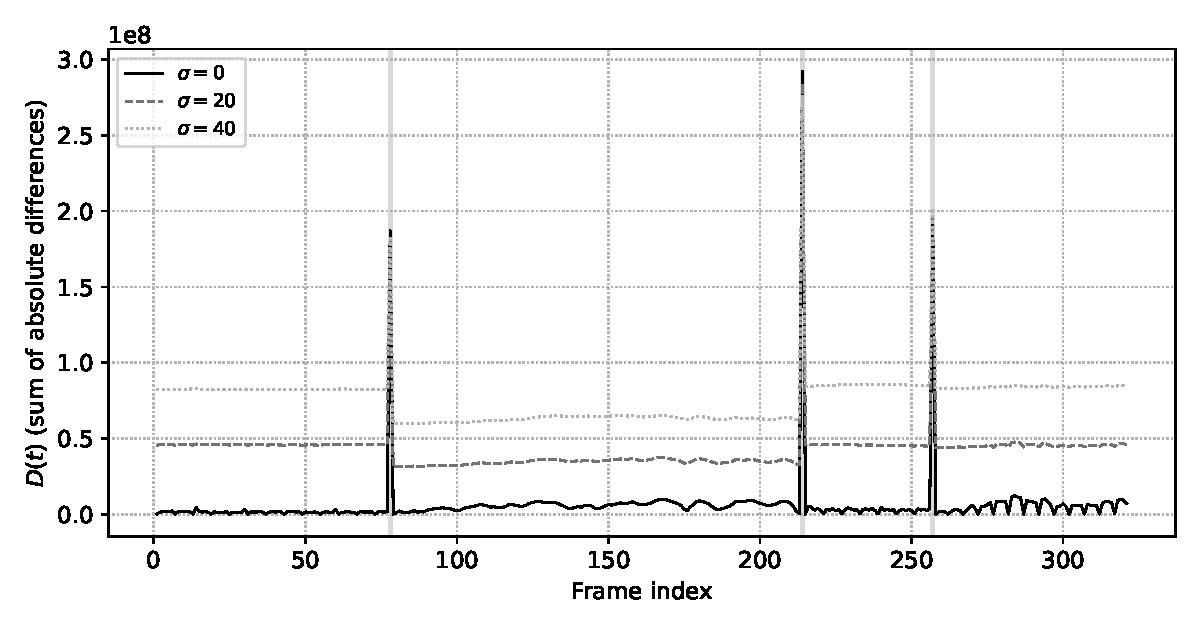
\includegraphics[width=0.95\linewidth]{../experiments/figures/exp04_noise_series.pdf}
\caption{ノイズ標準偏差 $\sigma = 0, 20, 40$ における変化量系列
$D(t)$。縦の薄い帯は正解の変わり目(フレーム 78, 214, 257)を示す。
ノイズは系列全体を上方へ平行移動させるが、ピークの高さはほとんど
変えない。}
\label{fig:b4-noise-series}
\end{figure}

\subsubsection{ノイズ頑健性の比較結果}

各ノイズ条件における方式 (1)(係数 $k = 3$)、方式 (3)
(窓幅 15、係数 4)、および後述のヒストグラム差分法
(平均 $+3\sigma_H$ 閾値)の評価結果を表 \ref{tab:b4-noise} に、
$F_1$ の推移を図 \ref{fig:b4-f1} に示す。

\begin{table}[htbp]
\centering
\caption{ノイズ標準偏差 $\sigma$ ごとの各方式の precision / recall / $F_1$
(正解 $\{78, 214, 257\}$、許容ずれ $\pm 1$ フレーム)}
\label{tab:b4-noise}
\begin{tabular}{r rrr rrr rrr}
\hline
& \multicolumn{3}{c}{方式 (1) 平均 $+3\sigma_D$}
& \multicolumn{3}{c}{方式 (3) 移動平均基準}
& \multicolumn{3}{c}{ヒストグラム差分} \\
$\sigma$ & prec. & rec. & $F_1$ & prec. & rec. & $F_1$ & prec. & rec. & $F_1$ \\
\hline
0 & 1.000 & 1.000 & 1.000 & 1.000 & 1.000 & 1.000 & 1.000 & 1.000 & 1.000 \\
5 & 1.000 & 1.000 & 1.000 & 1.000 & 1.000 & 1.000 & 1.000 & 1.000 & 1.000 \\
10 & 1.000 & 1.000 & 1.000 & 1.000 & 1.000 & 1.000 & 1.000 & 1.000 & 1.000 \\
20 & 1.000 & 1.000 & 1.000 & 1.000 & 0.333 & 0.500 & 1.000 & 1.000 & 1.000 \\
40 & 1.000 & 1.000 & 1.000 & 0.000 & 0.000 & 0.000 & 1.000 & 1.000 & 1.000 \\
\hline
\end{tabular}
\end{table}

\begin{figure}[htbp]
\centering
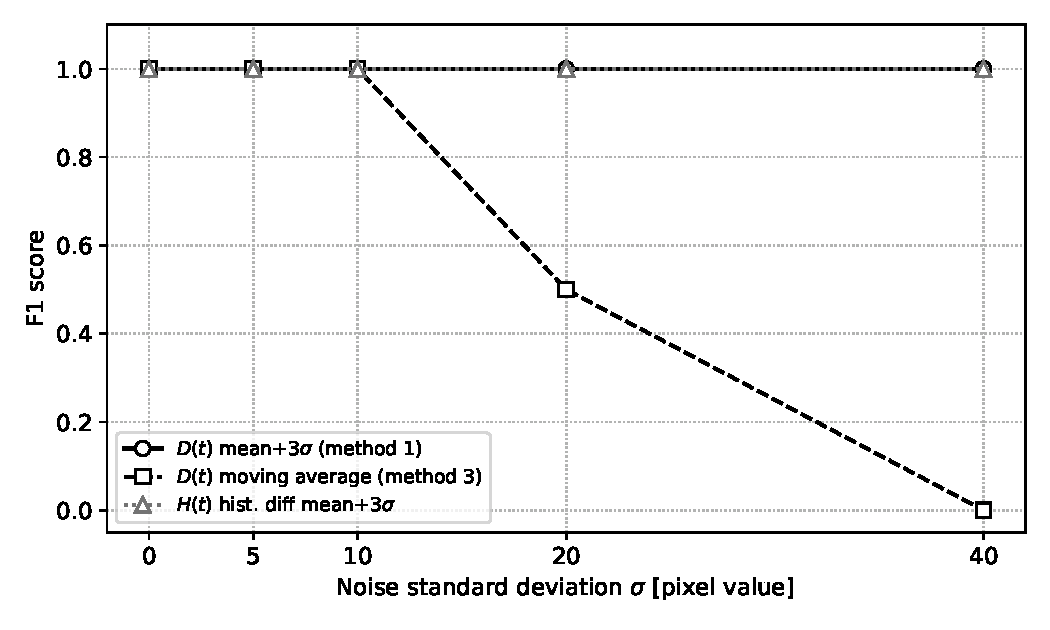
\includegraphics[width=0.8\linewidth]{../experiments/figures/exp04_f1_vs_sigma.pdf}
\caption{ノイズ標準偏差 $\sigma$ に対する各方式の $F_1$ スコア。
方式 (1) とヒストグラム差分法は全条件で $F_1 = 1.000$ を維持するが、
方式 (3) は $\sigma = 20$ 以上で急落する。}
\label{fig:b4-f1}
\end{figure}

方式 (1) は $\sigma = 40$ でも $F_1 = 1.000$ を維持した。これは
閾値 $\mu_D + 3\sigma_D$ の構造による。表 \ref{tab:b4-series} の
とおり、ノイズによるオフセットは $\mu_D$ に全額が反映される一方、
$\sigma_D$ はほぼ変化しない。したがって閾値はオフセットとともに
自動的に上方へ移動し($\sigma = 0$ の $7.17 \times 10^7$ から
$\sigma = 40$ の $1.29 \times 10^8$ へ)、ピークと床の間に
とどまり続ける。「系列との差」に基づく閾値は、系列全体への加法的な
撹乱と共変するため頑健である。

一方、方式 (3) は $\sigma = 10$ までは $F_1 = 1.000$ を維持したが、
$\sigma = 20$ で検出がフレーム 214 のみとなり
recall $= 0.333$($F_1 = 0.500$)、$\sigma = 40$ では 3 境界とも
検出できず $F_1 = 0$ となった。この失敗は方式 (3) の判定条件が
「移動平均基準線との比」であることから定量的に説明できる。ピーク値
$P$、基準線の値 $B$ の点にオフセット $c$ が加わると、判定に使われる
比は

\begin{equation}\label{eq:b4-ratio}
r(c) = \frac{P + c}{B + c}
\end{equation}

となり、$P > B$ のとき $r(c)$ は $c$ の単調減少関数で、
$c \to \infty$ で 1 に収束する。すなわち加法的ノイズは比に基づく
判定を必ず不利にする。表 \ref{tab:b4-ratio} に、各境界における
$D(t)$ と移動平均基準線の比の実測値を示す。判定条件は
「比が係数 4 を超えること」であるから、表中の値と 4 との大小関係が
そのまま表 \ref{tab:b4-noise} の検出結果に対応している。
$\sigma = 20$ では フレーム 214 の比 5.022 だけが 4 を超え、
フレーム 78(3.752)と 257(3.561)はわずかに下回って見逃された。
$\sigma = 40$ では最大のピークでも 3.155 となり全滅した。

\begin{table}[htbp]
\centering
\caption{各境界における $D(t)$ と移動平均基準線(窓幅 15)の比。
方式 (3) は比が 4 を超えた境界のみを検出する。}
\label{tab:b4-ratio}
\begin{tabular}{rrrr}
\hline
$\sigma$ & フレーム 78 & フレーム 214 & フレーム 257 \\
\hline
0 & 13.722 & 12.462 & 13.105 \\
5 & 8.362 & 9.382 & 7.996 \\
10 & 5.908 & 7.289 & 5.593 \\
20 & 3.752 & 5.022 & 3.561 \\
40 & 2.318 & 3.155 & 2.182 \\
\hline
\end{tabular}
\end{table}

先の定性的な考察では、動きの激しさが場所により異なる映像に対して、
閾値が局所的な変化量に追従する方式 (3) が最も頑健であると
位置付けた。本実験はこの結論に重要な限定を加える。方式 (3) の頑健性は
「局所的・乗法的な変動」に対するものであり、ノイズのように系列全体へ
一様に加算される撹乱に対しては、比の構造(式 \ref{eq:b4-ratio})が
災いして 3 方式の中で最も脆弱になる。逆に方式 (1) は全域で単一の
閾値しか持たないという弱点の裏返しとして、全域一様なオフセットには
完全に追従する。すなわち両方式の頑健性は撹乱の種類(局所的な変動か、
全域的なオフセットか)に対して相補的であり、どちらが優れているかは
入力に想定する劣化モデルに依存する。方式 (3) を加法的ノイズにも
頑健にするには、判定条件を「基準線の $k$ 倍」から「局所平均
$+ k \times$ 局所標準偏差」のような差に基づく形へ変更することが
有効と考えられる。

\subsubsection{係数 $k$ の感度と安全な範囲}

方式 (1) の係数 $k$ を 0.5 から 6.0 まで 0.25 刻み(23 点)で変化させ、
ノイズなしと $\sigma = 20$ の 2 条件で precision・recall・$F_1$ を
計測した。結果を図 \ref{fig:b4-k} に示す。両条件とも、走査した
すべての $k$ で検出数 3・$F_1 = 1.000$ であった。すなわち実測上の
安全な範囲は少なくとも $0.50 \le k \le 6.00$ であり、採用値 $k = 3$ は
この範囲の中央付近に位置する。

\begin{figure}[htbp]
\centering
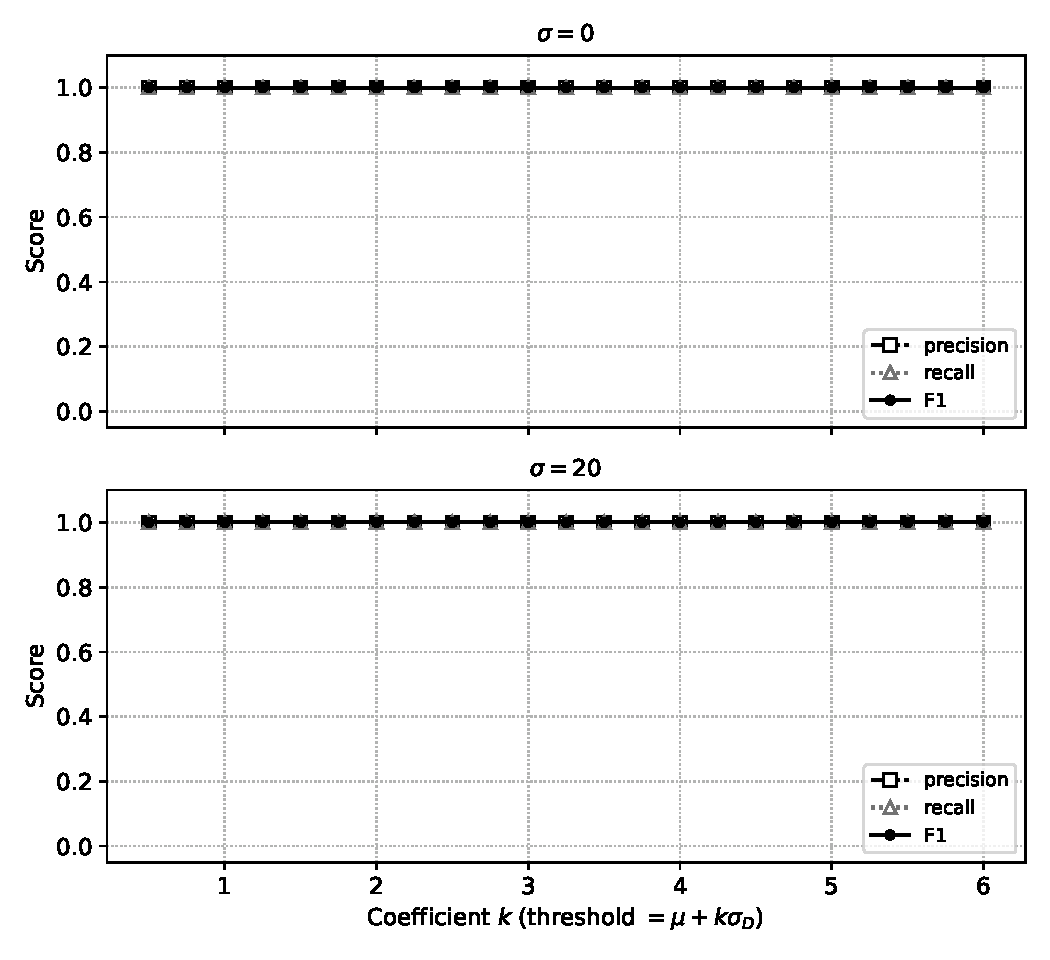
\includegraphics[width=0.85\linewidth]{../experiments/figures/exp04_k_sensitivity.pdf}
\caption{方式 (1) の係数 $k$ に対する precision・recall・$F_1$
(上: ノイズなし、下: $\sigma = 20$)。走査範囲
$0.5 \le k \le 6.0$ の全点で 3 指標とも 1.000 であった。}
\label{fig:b4-k}
\end{figure}

安全な範囲の限界は分離度から解析的に求められる。変わり目の集合を
$\mathcal{B}$ とすると、$F_1 = 1$ となる条件は閾値
$\mu_D + k\sigma_D$ が「非ピークの最大値以上、ピークの最小値未満」に
あることであり、その $k$ の下限と上限は

\begin{equation}\label{eq:b4-krange}
k_{\mathrm{low}} = \frac{\displaystyle \max_{t \notin \mathcal{B}} D(t)
- \mu_D}{\sigma_D}, \qquad
k_{\mathrm{high}} = \frac{\displaystyle \min_{t \in \mathcal{B}} D(t)
- \mu_D}{\sigma_D}
\end{equation}

で与えられる。実測系列から計算した $k$ の理論範囲を
表 \ref{tab:b4-krange} に示す。ノイズなしでは
$0.273 \le k < 8.276$ と極めて広く、$\sigma$ の増加とともに範囲は
狭まるが、最悪の $\sigma = 40$ でも $0.536 \le k < 5.969$ を保つ。
これは上位 3 ピークの最小値と非ピーク最大値の分離比が、ノイズなしの
15.40 から $\sigma = 40$ の 2.12 まで縮小してもなお 1 を大きく
超えているためである。採用値 $k = 3$ は全条件の範囲に含まれ、
かつ各範囲のほぼ中央にあることから、パラメータ選択として妥当で
あったと結論できる。ただしこの広い裕度は、本動画の変わり目がすべて
画面全体が入れ替わるハードカットであることに依存しており、変化量の
小さい境界(画面の一部のみの転換や緩やかな遷移)を含む映像では
$k_{\mathrm{high}}$ が下がり、安全な範囲は狭くなると考えられる。

\begin{table}[htbp]
\centering
\caption{分離度と、$F_1 = 1$ を与える係数 $k$ の理論範囲
(式 \ref{eq:b4-krange})。分離比は上位 3 ピークの最小値と
非ピーク最大値の比である。}
\label{tab:b4-krange}
\begin{tabular}{r rrr rrr}
\hline
& \multicolumn{3}{c}{$D(t)$(画素差分)}
& \multicolumn{3}{c}{$H(t)$(ヒストグラム差分)} \\
$\sigma$ & 分離比 & $k_{\mathrm{low}}$ & $k_{\mathrm{high}}$
& 分離比 & $k_{\mathrm{low}}$ & $k_{\mathrm{high}}$ \\
\hline
0 & 15.40 & 0.273 & 8.276 & 5.17 & 0.871 & 5.441 \\
5 & 9.74 & 0.209 & 8.182 & 7.53 & 0.524 & 5.255 \\
10 & 6.49 & 0.207 & 7.982 & 8.91 & 0.407 & 5.173 \\
20 & 3.78 & 0.274 & 7.405 & 13.69 & 0.211 & 5.413 \\
40 & 2.12 & 0.536 & 5.969 & 18.16 & 0.136 & 6.333 \\
\hline
\end{tabular}
\end{table}

\subsubsection{ヒストグラム差分法との比較}

比較手法として、フレームの空間情報を捨てて明るさの分布だけを
比較するヒストグラム差分法を追加実装した。各フレームの 64 ビン
正規化グレースケールヒストグラム $h_t(b)$ に対し、隣接フレーム間の
L1 距離

\begin{equation}\label{eq:b4-hist}
H(t) = \sum_{b=0}^{63} \bigl| h_t(b) - h_{t-1}(b) \bigr|
\end{equation}

を系列として用いる。ノイズなしの条件で、$H(t)$ の上位 3 ピークは
$\{78, 214, 257\}$ となり $D(t)$ と完全に一致した。平均
$+3\sigma_H$ 閾値でも同じ 3 フレームのみが検出され、
$F_1 = 1.000$ である。さらに表 \ref{tab:b4-noise} のとおり、
ヒストグラム差分法は $\sigma = 40$ までの全ノイズ条件で
$F_1 = 1.000$ を維持した。図 \ref{fig:b4-series} に両系列の対比を
示す。

\begin{figure}[htbp]
\centering
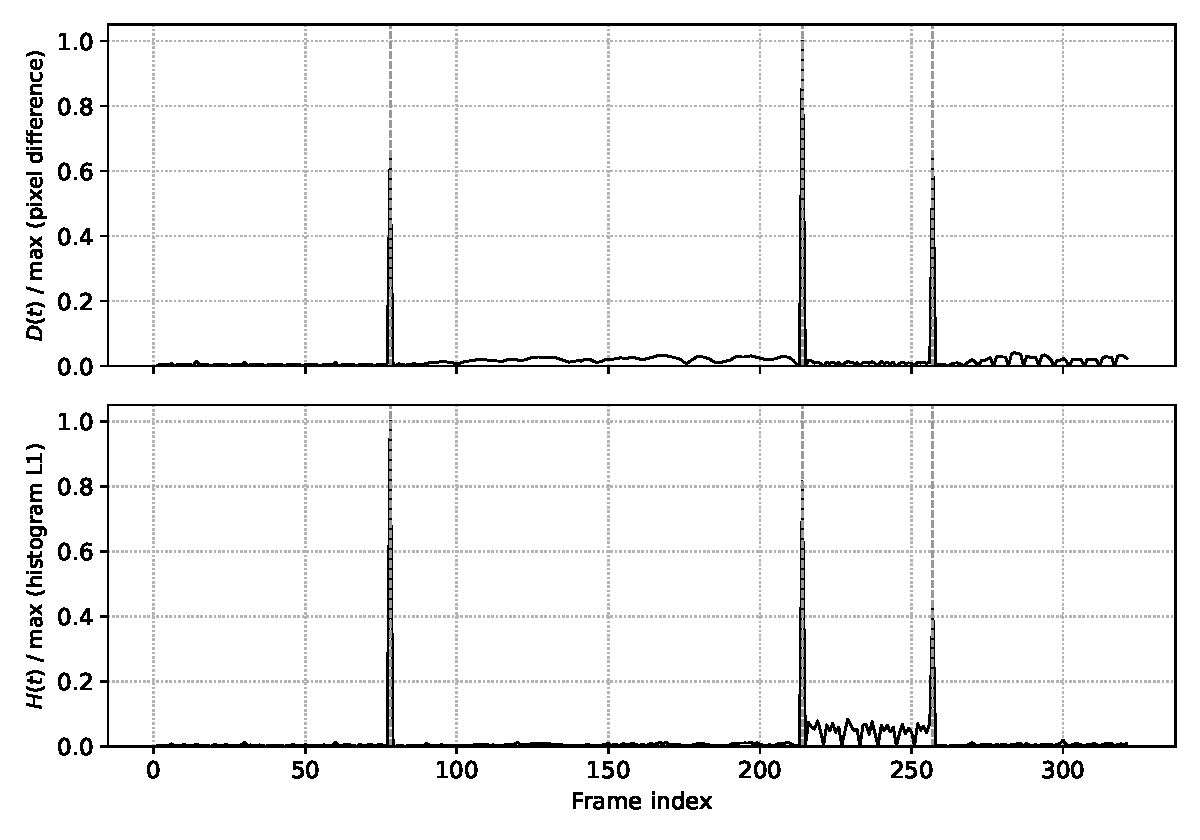
\includegraphics[width=0.95\linewidth]{../experiments/figures/exp04_series_compare.pdf}
\caption{画素差分系列 $D(t)$(上)とヒストグラム差分系列 $H(t)$(下)
の対比(ノイズなし、いずれも最大値で正規化)。縦の破線は正解の
変わり目を示す。両系列とも 3 境界で明瞭なピークを持つ。}
\label{fig:b4-series}
\end{figure}

両手法の違いは分離度のノイズ依存性に現れる(表 \ref{tab:b4-krange})。
ノイズなしでは $D(t)$ の分離比 15.40 に対して $H(t)$ は 5.17 であり、
画素差分の方が境界を鋭く分離する。これは図 \ref{fig:b4-series} の
下段でフレーム 214〜257 の区間の $H(t)$ が相対的に大きく変動している
(非ピーク最大値 0.135 はこの区間にある)ことに対応し、この
ショット内の明るさ分布の変動をヒストグラム差分が拾うためである。
ところがノイズを加えると関係は逆転し、$\sigma = 40$ では $D(t)$ の
分離比が 2.12 まで悪化するのに対し、$H(t)$ の分離比はむしろ 18.16 へ
改善する。ヒストグラムは画素の空間的対応を取らずに分布を比較する
ため、ゼロ平均のノイズは隣接 2 フレームのヒストグラムを「同じ形に
平滑化する」だけで、差分にはほとんど寄与しない。実際、$H(t)$ の
平均はノイズなしの $2.78 \times 10^{-2}$ から $\sigma = 40$ の
$1.26 \times 10^{-2}$ へと逆に減少しており、ノイズによる平滑化が
ショット内の細かい分布差を均していることが分かる。

以上から、両手法にはノイズ頑健性と識別力のトレードオフがある。
画素差分 $D(t)$ は空間情報を保持するため、明るさ分布が同じまま
構図だけが変わる境界も原理的に検出できるが、画素単位のノイズが
式 \ref{eq:b4-offset} のオフセットとして全額加算される。
ヒストグラム差分 $H(t)$ はゼロ平均ノイズにほぼ不変である代わりに、
明るさ分布の似た場面間の境界を原理的に検出できない。いずれも
1 フレームあたりの計算量は画素数に対して線形であり、計算コストの
差は小さいことから、両系列を併用して「いずれかが閾値を超えた
フレーム」を境界候補とする構成も現実的な改善案である。

\subsubsection{古典手法の適用範囲と深層学習手法の位置付け}

本実験の結果は、ハードカットのみで構成された映像に対しては、
フレーム間差分と統計的閾値という古典的構成で完全な検出
($F_1 = 1.000$)が達成でき、しかもパラメータ裕度が広く
($0.5 \le k \le 6.0$)、強いノイズ($\sigma = 40$)にも方式の
選択次第で耐えることを示した。一方で、実際の映像に含まれる
ディゾルブやフェードのような緩やかな遷移では、変化量が多数の
フレームに分散するため $D(t)$ に明瞭なピークが立たず、単一フレームの
閾値判定は原理的に不利になる。近年のショット境界検出研究はこの
領域を深層学習で扱っており、Sou\v{c}ek らの TransNet V2 は
3 次元畳み込みネットワークにより急峻な遷移と緩やかな遷移の両方を
学習ベースで検出し、標準ベンチマークで最高水準の性能を報告している
\cite{b4-transnetv2}。また Zhu らは短尺動画 853 本・11606 個の
ショット境界を注釈したデータセット SHOT を構築し、ニューラル
アーキテクチャ探索を用いた AutoShot により TransNet V2 を
$F_1$ で 4.2 ポイント上回る結果を報告している \cite{b4-autoshot}。

これらの深層学習手法は学習データと計算資源を要するのに対し、
本課題の手法は無学習・パラメータ 1 個・フレームあたり線形時間で
動作する。本実験で示したとおり、対象がハードカット主体であれば
古典手法で十分な精度と裕度が得られるため、手法の複雑さは対象映像に
含まれる遷移の種類(ハードカットのみか、緩やかな遷移を含むか)に
応じて選択すべきである。
